\def\dt{\,\text{dt}\,}
\def\dx{\,\text{dx}\,}
\def\dk{\,\text{dk}\,}
\chapter{Vorbereitung}
    \section{Fourierreihen und -transformation}
Die Fourier-Analysis findet gerade in der Optik häufig Anwendung. Im Kontext der 
Holografie stellen vor allem Fourierreihen und die Fouriertransformation nützliche
Hilfsmittel dar, weshalb diese zur Vorbereitung näher betrachtet werden sollen.
    \subsection*{Fourierreihenentwicklung}
Die Fourierreihe bietet die Möglichkeit einen großen Teil der periodischen 
Funktionen durch eine Linearkombination von Sinus- und Kosinustermen verschiedener
Frequenzen und Amplituden zu entwickeln.
        \begin{align*}
           f(t) = \sum_{k=0}^\infty a_k \cos(\omega_k \, t) + b_k \sin(\omega_k \, t) 
           \qquad \text{mit  } \omega_k =  \frac{2 \pi k}{T}
        \end{align*}
$T$ sei hierbei die Periodendauer der Funktion. Die \emph{Fourierkoeffizienten} $a_k$
und $b_k$ werden hier beschrieben durch
        \begin{align*}
            a_0 = \frac{1}{T} \int_{-T/2}^{+T/2} f(t) \dt \quad &a_k = \frac{2}{T} \int_{-T/2}^{+T/2} f(t) \cos(\omega_k \, t) \dt \;(k\neq 0)\\
            &b_k = \frac{2}{T} \int_{-T/2}^{+T/2} f(t) \sin()\omega_k \, t) \dt
        \end{align*}
Dies soll nun an zwei wichtigen Funktionen demonstriert werden.
            \subsubsection*{Rechtecksfunktion}
        \begin{wrapfigure}{r}{0.45\textwidth}
            \vspace{10pt}
            \centering
            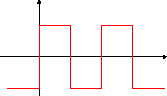
\includegraphics[width=0.4\textwidth]{Abb/rechteck.pdf}
            \caption{Rechtecksfunktion}
            \label{rechteck}
            \vspace{10pt}
        \end{wrapfigure}
Die Rechtecksfunktion ist gegeben durch
        \begin{align*}
            f(t) = \begin{cases}
                -1 & \text{für } -1 < t < 0 \\
                 1 & \text{für }  0 < t < 1
            \end{cases}   
        \end{align*}
mit periodischer Fortsetzung.\\
Um nun die Fourierreihendarstellung nutzen zu können, müssen zuerst die Koeffizienten
errechnet werden. Für $T=2$ ergibt sich:
        \begin{itemize}
            \item da die Rechtecksfunktion eine ungerade Funktion ist gilt $a_k = 0$
            \item für die $b_k$ gilt
                \begin{align*}
                   b_k &=\frac{2}{2} \int_{-1}^{1} f(t) \sin(\pi k t ) \dt = 
                   \int_{-1}^{0} - \sin(\omega_k t) \dt 
                   + \int_0^1 \sin(\omega_k t ) \dt \\
                   &= \frac{1}{\pi k} \left[
                       \left(1 - \cos
                        \left(-\frac{\pi k}{2}
                        \right)
                       \right)
                     + \left(-\cos
                        \left( \frac{\pi k}{2}
                        \right) + 1
                       \right)
                    \right]
                    = \frac{2}{\pi k} \left( 1 + \cos(\pi k)\right)
                \end{align*}
            \end{itemize}
Somit erhalten wir für die Fourierreihenentwicklung der Rechtecksfunktion
                \begin{align*}
                   f(t) = \sum_{k=0}^\infty \frac{2}{\pi k} (1 + \cos(\pi k)) 
                   \sin(\pi k t) 
                \end{align*}
                \begin{figure}[htbp]
                  \begin{minipage}{0.45\textwidth}
                   \centering
                    \includegraphics[width=0.9\textwidth]{Abb/rechteck_10}
                    \caption{Die Rechtecksfunktion bis zum 10. Summanden entwickelt}
                    \label{rechteck_10}
                  \end{minipage}\hfill
                  \begin{minipage}{0.45\textwidth}
                   \centering
                    \includegraphics[width=0.9\textwidth]{Abb/rechteck_1000.pdf}
                    \caption{Die Rechtecksfunktion bis zum 1000. Summanden entwickelt}
                    \label{reckteck_1000}
                  \end{minipage}
                \end{figure}
In Abbildung \ref{rechteck} ist die Reihenentwicklung bis zum 100000. Glied 
geplottet, während in Abbildung \ref{rechteck_10} und \ref{reckteck_1000} bis zur 
10. und 1000. Ordnung geplottet wurde. 

                    \subsubsection*{Dreiecksfunktion}
            \begin{wrapfigure}{r}{0.45\textwidth}
                \vspace{10pt}
                \centering
                \includegraphics[width=0.4\textwidth]{Abb/dreieck.pdf}
                \caption{Rechtecksfunktion}
                \label{dreieck}
                \vspace{10pt}
            \end{wrapfigure}

Die Dreiecksfunktion ist gegeben durch
                \begin{align*}
                   g(t) = \begin{cases}
                    -2(x+1) & \text{für } -1   < t < -0,5 \\
                    2x      & \text{für } -0,5 < t <  0,5 \\
                    2(x+1)  & \text{für } 0,5  < t <  1
                        \end{cases}
                \end{align*}
auch hier mit periodischer Fortsetzung.
Wiederum müssen die Koeffizienten berechnet werden:
                \begin{itemize}
                   \item es handelt sich um eine ungerade Funktion, also $a_k = 0$
                   \item die $b_k$ ergeben sich zu:
                        \begin{align*}
                            b_k &= \int_{-1}^{-1/2} -2(x+1) \sin(\omega_k t) \dt
                            + \int_{-1/2}^{1/2} 2 \, x \sin(\omega_k t) \dt
                            + \int_{1/2}^{1} 2(1-x) \sin(\omega_k t) \dt \\
                            &= \dots = \frac{4}{\pi^2 k^2}  
                             \left(
                                2 \sin \left( \frac{\pi \,k}{2} \right)
                                - \sin(\pi \, k)
                             \right)
                        \end{align*} 
                \end{itemize}
Die Fourierreihe ergibt sich also zu:
                \begin{align*}
                   g(t) = \sum_{k=0}^\infty \frac{4}{\pi^2 k^2} 
                    \left(
                        2 \sin \left( \frac{\pi \, k}{2} \right)
                        - \sin(\pi \, k) 
                    \right) \cdot \sin(\pi \, k \, t) 
                \end{align*}
                \begin{figure}[htbp]
                  \begin{minipage}{0.45\textwidth}
                   \centering
                    \includegraphics[width=0.9\textwidth]{Abb/dreieck_1}
                    \caption{Die Dreiecksfunktion bis zum 1. Summanden entwickelt}
                    \label{dreieck_1}
                  \end{minipage}\hfill
                  \begin{minipage}{0.45\textwidth}
                   \centering
                    \includegraphics[width=0.9\textwidth]{Abb/dreieck_10.pdf}
                    \caption{Die Dreiecksfunktion bis zum 10. Summanden entwickelt}
                    \label{dreieck_10}
                  \end{minipage}
                \end{figure}
Für Abbildung \ref{dreieck} wurde nur bis zum 1000. Summenglied geplottet. Man sieht
also, dass diese Funktion auch mit weniger Rechenaufwand gut genähert werden kann.
Bei sehr kleinen Ordnungen ist lediglich die Spitze, wie in Abbildung \ref{dreieck_10}
und vor allem in \ref{dreieck_1} zu sehen, noch sehr rundlich.

        \subsection*{Fouriertransformation}
Die Fouriertransformation stellt den Übergang der diskreten Fourierreihe zum
kontinuierlichen Integral dar. Diese erlaubt weiter die Darstellung nicht-periodischer
Funktionen. Für alle integrierbaren Funktionen ist sie definiert als
                \begin{align*}
                   F(f)(k) &= \frac{1}{(2\pi)^{n/2}} \int_{\mathbb{R}^n}
                    f(x) \cdot e^{-ikx} \dx & &\text{\textbf{Hintransformation}}\\
                    f(x) &= \frac{1}{(2\pi)^{n/2}} \int_{\mathbb{R}^n}
                    F(f)(k) \cdot e^{-ikx} \dk & &\text{\textbf{Rücktransformation}}
                \end{align*}
Durch die Fouriertransformation lässt sich eine Funktion über eine ihr zugehörige
andere Variable darstellen. Beispiele hierfür sind Ort $x$ und Wellenzahl $k$,
oder Zeit $t$ und Frequenz $\omega$.